\documentclass[12pt]{dalthesis}
\usepackage{amsmath,graphicx,braket}

\begin{document}

\title{An investigation into the properties of a physical adiabatic quantum computer}
\author{Elliot Snow-Kropla}
%\date{20 July 2012}

\degree{Master of Science}
\degreeinitial{M.Sc.}
\faculty{Faculty of Science}
\dept{Department of Physics and Atmospheric Science}

\defencemonth{August}\defenceyear{2014}

\frontmatter

\begin{abstract}

\end{abstract}

\begin{acknowledgements}
\end{acknowledgements}

\mainmatter

\chapter{Introduction}

\section{Classical Computing}

\section{Feynman to Shor}

\section{The Adiabatic Theorem}
The adiabatic theorem states that if a system is initially prepared in the $ith$ energy level, and the Hamiltonian is evolved according to the adiabatic condition, the system will remain in the $ith$ state after the evolution.  The adiabatic condition is given as:

\begin{displaymath}
	\left | \frac{1}{\omega_{fi}}\frac{\partial}{\partial t} \braket{\psi_f | \hat{V}(t) | \psi_i} \right | << |E_f - E_i|
\end{displaymath}

where $E_i$ and $E_f$ are the energies of the initial and final states, $\hat{V}(t)$ is the time dependant part of the Hamiltonian and $\omega_{if} = \frac{E_f - E_i}{\hbar}$ is a convenient variable.  This (FIXME missing!) derivation due to \cite{zettili}.

\chapter{Adiabatic Quantum Computing}
\section{Literature Survey}
Introduced by Farhi et.\ al.\cite{farhi}, the idea of adiabatic quantum computation (hereafter AQC) is to exploit the adiabatic theorem to solve computational problems.  There are two main components to the idea.  First, we find a Hamiltonian such that the ground state is the solution to a computational problem (e.g. a bitstring of spins pointed up and down).  Second, we use the adiabatic theorem to move from some easily prepared initial state into the Hamiltonian we found.

\section{Finding a Problem Hamiltonian}
While in principle there are an unlimited number of ways to construct a Hamiltonian whose ground state encodes the solution to a computation, our method is to use an N-particle Hamiltonian of the form

\begin{displaymath}
	H = \sum_{i} h_i \sigma_i^Z + \sum_{i < j} J_{ij} \sigma_i^Z\sigma_j^Z 
\end{displaymath}
where $\sigma_i^Z$ is the pauli matrix of the ith particle and $h_i$ and $J_{ij}$ are the parameters of the Hamiltonian.  This 2-local Hamiltonian corresponds to a graph structure, where each particle is a vertex and each non-zero $J_{ij}$ is an edge, while non-zero $h_i$s can be represented as edges to a constant "field" spin.

Our problem of finding a suitable Hamiltonian is now reduced to finding a set of $h$'s and $J_{ij}$'s such that our desired solution is encoded in the ground state.  We do this by breaking our problem down into sub-problems and finding Hamiltonians for these easier sub-problems, and then reassembling these smaller Hamiltonians into the final problem Hamiltonian using the gluing theorem.\cite{gluing}

Figure \ref{fig:nand_graph} shows a Hamiltonian graph describing the $h_i$'s and $J_{ij}$'s to encode the logic of a NAND gate.  Because NAND's are universal for computation, combining this graph with the gluing theorem allows us to encode the evaluation of any computable function into the ground state of a Hamiltonian of the general form we described above.  

\begin{figure}
	%\scalebox{}{
	%	\includegraphics[]{}
	%}
	\caption[\texttt{NAND} Graph]{Graphical representation of the Hamiltonian implementing the logic of a \texttt{NAND} gate.}
	\label{fig:nand_graph}
\end{figure}


We don't expect this encoding using NANDs glued together to be either optimal in the sense of using fewest spins or couplings, or to be asymptotically faster than an equivalent classical circuit.  We have no general solution for the first problem; each computational problem we want to encode efficiently requires it's own bespoke encoding.  To solve the second problem we take advantage of the fact that quantum mechanics is time-reversible: which variables are output and which are input is arbitrary.  Thus if we have a solution in mind for a given problem we can simply encode the Hamiltonian ``backwards'' and recover answers that would lead to our initial solution.  For NP problems, where verifying a solution is in P, we can thus write a verification circuit with a solution of \texttt{true} and find the inputs to our NP problem.

Our approach to solving NP problems is thus:
\begin{itemize}
	\item Construct a circuit to verify a candidate solution (for satisfiability this would be evaluation of the clauses; for factoring this would be a multiplication circuit)
	\item Clamp the ``output'' spins to their required values (for a satisfiability problem this would be all output spins \texttt{true}; for a factoring problem this the number to factor)
	\item Run the adiabatic computer and read off the ``input'' spins
\end{itemize}

\section{Adiabatic Evolution}

\chapter{Embedding}
Because in general programs compiled to Ising graphs can be of any shape, we need a way to convert arbitrary graphs into Chimera graphs that can be executed on a machine.  This is done by adding \emph{clone spins} into the graph: each clone spin has the same value in the ground state as one of the logical spins in the input graph.  Thus we can decrease the connectivity of the input graph until it is sparse enough to be isomorphic to a physical machine.

\section{ Embedding algorithm}

The embedding algorithm is as follows:

\emph{\textbf{Definitions:}}

Designate the input Hamiltonian graph $V$ and the output Chimera graph $G$.  Label the spins in $V$ and $G$ as $V_i$ and $G_i$ respectively.
We define the \emph{clone map} $C_i$ as the set of spins $[i,j \ldots]$ which have the same logical value as their parent spin: so for example the clone map of spin 5, $C_5$, might be $[2,3,13]$ which would mean that spins 2, 3, 5 and 13 all share the same logical value.  We define a mapping $M$ between logical spins in graph $V$ and computation spins in graph $G$.  

We also define a \emph{clone coupling} value which is as large as possible and ferromagnetic; this attempts to ensure that all the members of a clone map are aligned in the ground state.  In the final $G$, each member of a clone map should have a clone coupling connecting it to at least one other member of the clone map.

\emph{\textbf{Procedure:}}
\begin{enumerate}
	\item Populate $M$ by mapping each $V_i$ to one of the spins $G_j$ on the left side of a qubyte that lies along the diagonal of $G$
	\item For each field term in $V$, add a field to $G$ on the corresponding spin
	\item For each $J_{ij}$ in $V$, conduct the following operation:
		\begin{itemize}
			\item Scan through both of $C_i$ and $C_j$ to find the pair which are nearest to each other in $G$; call these $x$ and $y$
			\item Get a list of each spin that lies along the path between $x$ and $y$
			\item Assign half of these spins to $C_i$ and half to $C_j$; add the appropriate clone coupling into $G$ for each spin in the path to ensure that the clone map is properly connected
			\item Finally, at the interface between the two new clone map members, add a coupling into $G$ with the same value as $J_{ij}$
		\end{itemize}
\end{enumerate}

Each term in $V$, both fields and couplings, should now have a corresponding term in $G$.  $G$ should also contain many coupling terms that group the necessary clone maps.

\chapter{The \texttt{VESUVIUS} Machine}

\section{Resolution}
In addition to the graph-shape restrictions, the \texttt{VESUVIUS} machine cannot implement arbitrary physical Hamiltonians.  The machine can only implement fields and couplings as one of 15 distinct values: $-7/7, -6/7 \dots 5/7,6/7, 7/7$.  As our embedded Hamiltonians don't generally have these coupling values, they must be manipulated to fit in this range.

\chapter{Preliminary Results}

\begin{figure}[h]
	\scalebox{0.6}{
	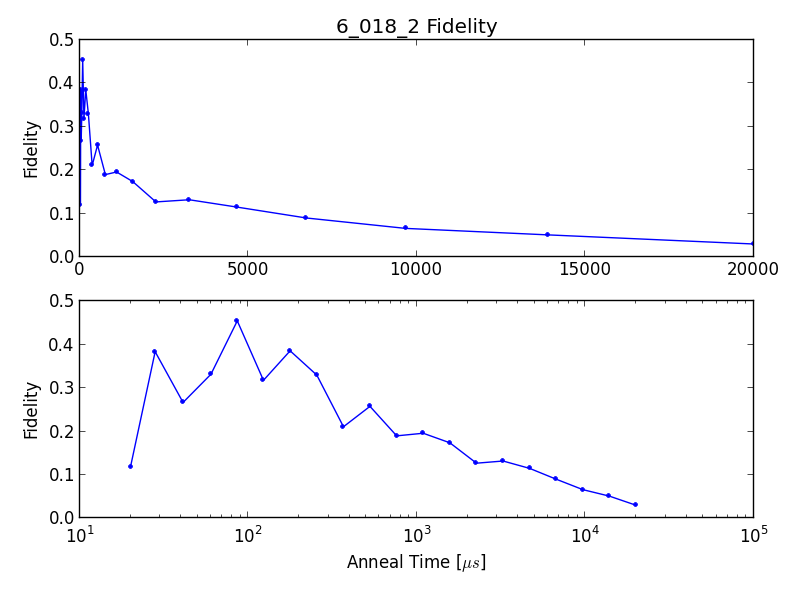
\includegraphics[bb=0 0 800 600]{img/6_018_2_fidelity.png}
}
	\caption[Fidelity vs Time]{Plot of the fidelity as a function of annealing time for the Hamiltonian ``6\_018'' both linear and log-scaled x-axis.}
	\label{fig:fidelity}
\end{figure}

Figure \ref{fig:fidelity} shows the results of 50,000 runs of the annealing machine consisting of 50 runs with 1000 reads at various annealing times.  Along the y-axis is the fidelity, and along the x-axis is the annealing time.  Contrary to what we expect from the adiabatic theorem and simulations of quantum annealing the fidelity is uncorrelated with annealing from 20$\mu$s out to roughly 500$ \mu$s, after which the fidelity \emph{decreases} with increasing annealing time.  This unexpected behaviour leaves us with a number of questions:

\begin{itemize}
	\item For short annealing times, why does the fidelity appear insensitive to annealing time?
	\item For long annealing times, why does the fidelity decrease with increasing annealing times?
	\item Is the short time fidelity dominated by the Hamiltonian programming noise?
	\item Is there significant drift in the fidelities after programming (i.e. read noise)?
	\item Does the Hamiltonian fidelity depend strongly on the number of coupling values?
\end{itemize}

or in short: Our theoretical model of quantum annealing suggests that the fidelity at T = 0 should be $2^{-N}$ for an $N$ spin Hamiltonian and increase as the annealing time increases, reaching approximately $1$ in the limit of $T \rightarrow \infty$ (as shown in Figure \ref{fig:simulated_anneal}).  Instead, the fidelity at our smallest accessible annealing time is already ``large'' and is seemingly insensitive to annealing time until the fidelity begins to \emph{drop} (as shown in Figure \ref{fig:fidelity}).

\emph{Why does the machine behave in this way contrary to our expectations?  Why does the short-anneal fidelity vary so much, and why does the long-anneal fidelity decrease rather than increase?}

\section{Short-time Evolution}
The data for short time evolution is inconsistent with the fidelity being a function of nothing but annealing time.  The fidelity between different runs varies significantly more than the standard deviation determined from averaging the reads.  Thus, there must be some other factor dominating the fidelity.  Options include:

\begin{itemize}
	\item Run noise in the machine: that is, each time the physical Hamiltonian is implemented the actual values of the fields and couplings are different, producing a different Hamiltonian every time.  This would mean that within a given run we see a consistent fidelity, but between runs we don't
	\item Our Hamiltonians might have too many coupling values, and resolution issues on the machine could be exacerbating the run noise
\end{itemize}

Our plan to resolve this question is to run smaller and simpler Hamiltonians until we can see smooth fidelity curves at small annealing times, or our Hamiltonians are so simple (i.e. 2-spin ferromagnetic ground states) that we are convinced the run noise is intrinsic.  By smaller and simpler, we mean (in order of increasing complexity):

\begin{itemize}
	\item Hamiltonians with no clones and \emph{no} couplings, only fields
	\item Hamiltonians with couplings lying in the range $\pm 1$
	\item Hamiltonians with clones
	\item Hamiltonians larger than a single k44
	\item Hamiltonians containing clone chains
\end{itemize}

\section{Long-time Evolution}
For a purely quantum system the fidelity should increase in the limit of increasing annealing time.  What we see instead in the actual data is that the fidelity appears to approach zero as the annealing time increases.  The physical computer is not an ideal quantum system, so to model it correctly we need to account for noise and decoherence sources.

We should fit this decreasing fidelity, or perhaps the population histogram, to some sort of model of thermal noise.  Then we could determine the energy leakage, maybe.







\begin{figure}
	\scalebox{0.35}{
		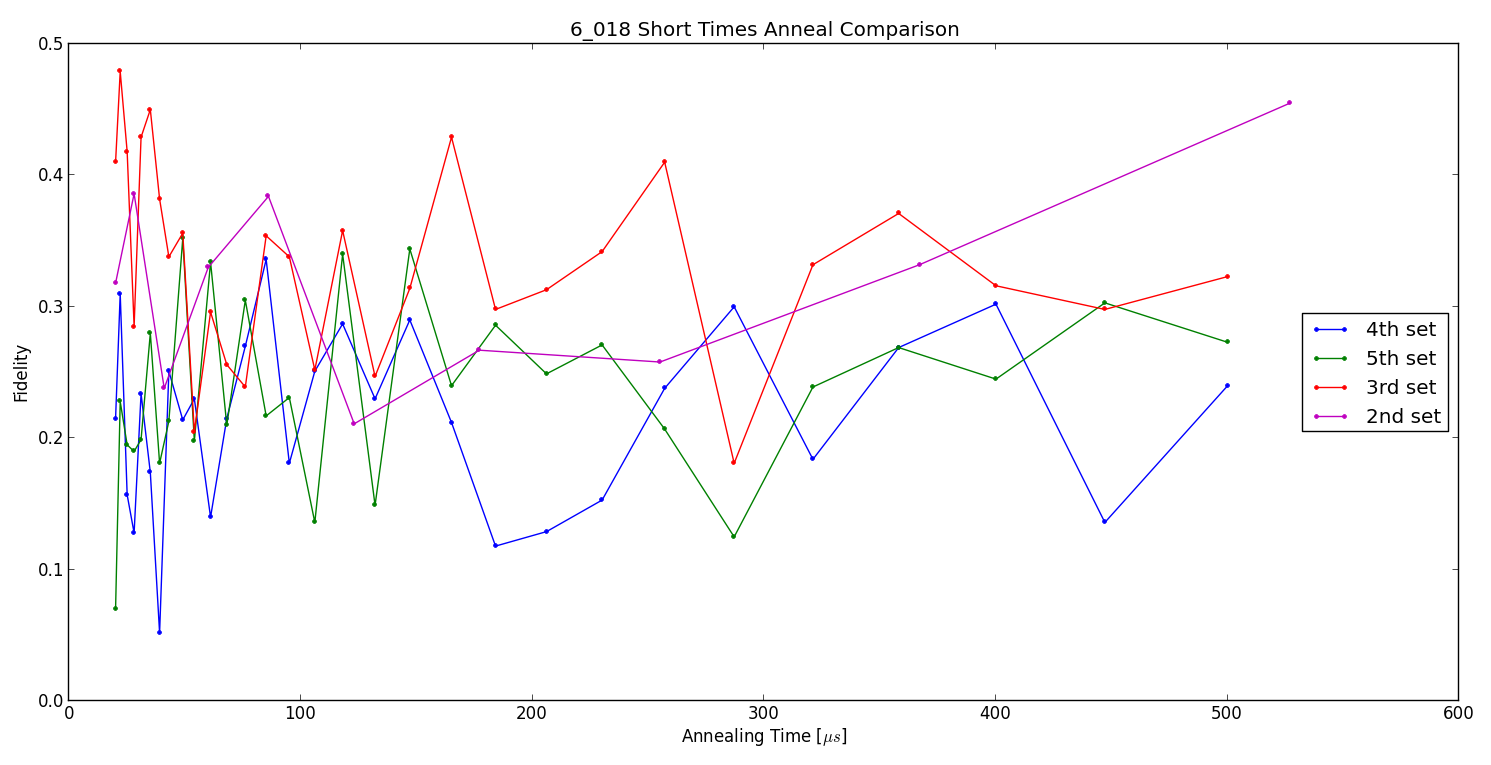
\includegraphics[bb= 0 0 745 382]{img/6_018_comparison.png}
	}
	\caption[Short Time Fidelities]{The fidelity as a function of time for the Hamiltonian ``6\_018'' for several different machine runs.  Each data point consist of 1000 machine reads.  Notice the spread between machine runs is outside of the error bars.}
	\label{fig:short_fidelity}
\end{figure}

\begin{figure}
	\scalebox{0.75}{
		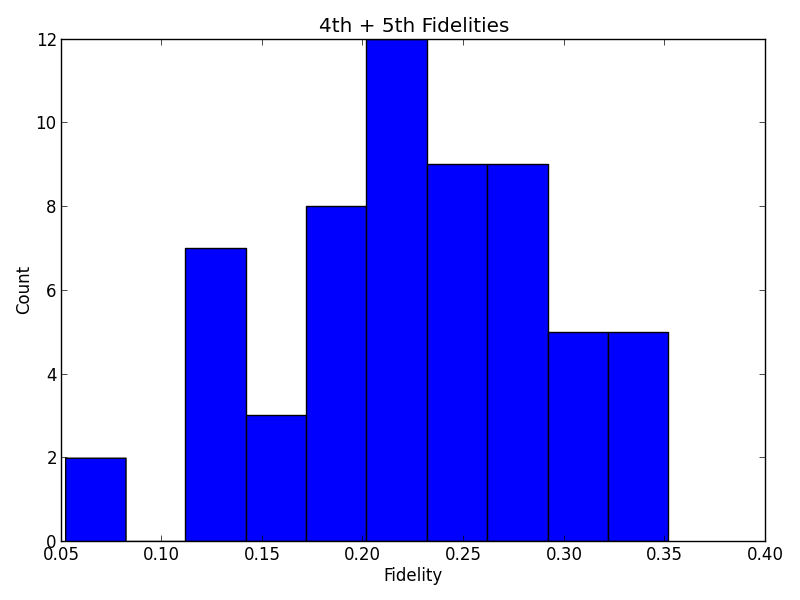
\includegraphics[bb= 0 0 800 600]{img/4_5_hist.png}
	}
	\caption[Short Time Fidelity Histogram]{Histogram of the fidelities found for all annealing times  $< 500 \mu$s.  Notice the gaussian like structure.}
	\label{fig:fid_hist}
\end{figure}

\begin{figure}
	%\scalebox{0.75}{
	%	\includegraphics[]{}
	%}
	\caption[Simulation of Schr\"odinger's Equation]{Numerical integration of Schr\"odinger's Equation for the Hamiltonian ``k44'' showing the fidelity increasing to a plateau as the annealing time increases.}
	\label{fig:simulated_anneal}
\end{figure}

\begin{figure}
	%\scalebox{0.75}{
	%	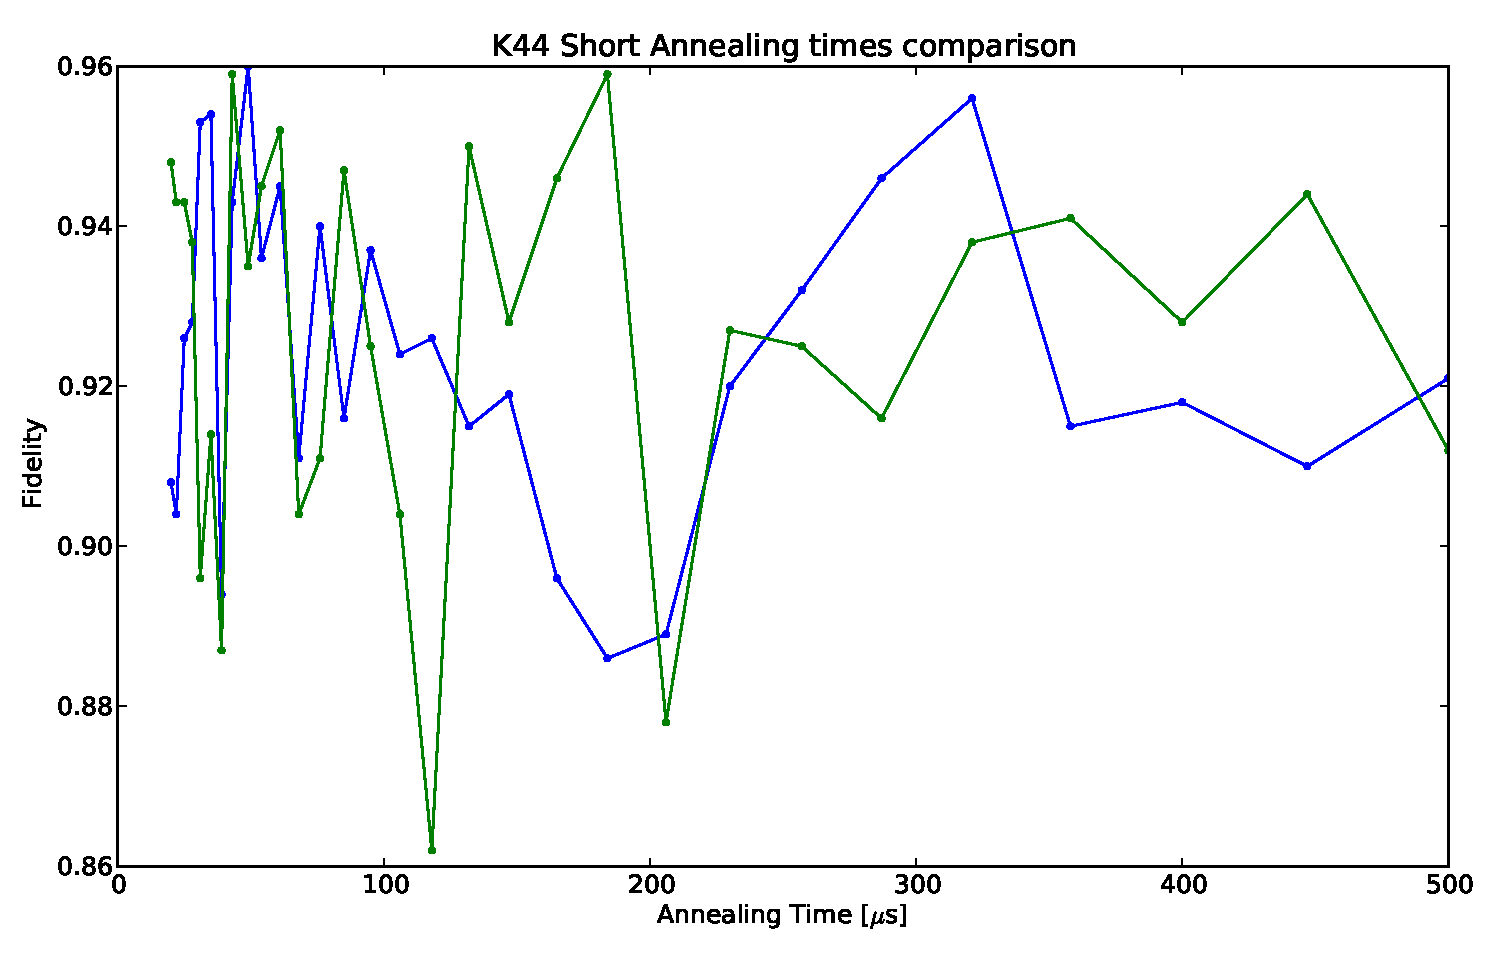
\includegraphics{img/k44_comparison.pdf}
	%}
	\caption[Long Time Anneal]{Machine data from Hamiltonian ``k44'' with 100 runs of 1000 reads showing the Hamiltonian noise at short times and the fidelity drop at long anneal times.}
	\label{fig:k44_long}
\end{figure}


\bibliographystyle{plain}
\bibliography{eskthesis}
\end{document}
